%%%% CAPÍTULO 4 - RESULTADOS E DISCUSSÃO
%%
%% Deve descrever detalhadamente os dados obtidos 
%% pelo autor. Normalmente são incluídas ilustrações
%% como: quadros, tabelas, gráficos, etc. Deve efetuar
%% a comparação dos dados obtidos e/ou resultados, com
%% aqueles descritos na revisão de literatura, 
%% incluindo os comentários sobre os estudos de outros
%% autores.

%% Título e rótulo de capítulo (rótulos não devem conter caracteres especiais, acentuados ou cedilha)
\chapter{Resultados e Discussão}\label{cap:resultadosediscussao}

% Deve descrever detalhadamente os dados obtidos pelo autor. Normalmente são incluídas ilustrações como: quadros, tabelas, gráficos, etc. Deve efetuar a comparação dos dados obtidos e/ou resultados, com aqueles descritos na revisão de literatura, incluindo os comentários sobre os estudos de outros autores.

\ric{Vamos organizar o capítulo da seguinte forma:}

\begin{enumerate}
    \item Análise exploratória: resultados estatísticos (visualizações) que permitam caracterizar de forma geral a base de dados utilizada;
    \item Operação da rede de transporte: resultados obtidos do uso de grafos temporais na caracterização da operação atual da rede de transporte de Curitiba;
    \item Integração temporal: resultados do estudo de uma integração temporal na rede de transporte de Curitiba
\end{enumerate}

\section{Análise exploratória}

Os resultados foram obtidos para o período de  01/03/2019 a 30/06/2019, tendo sido coletados 33 Gigabytes de dados, com 293.390.175 registros de geolocalização dos 1708 ônibus em operação. Este volume de dados gerou, após a transformação para o banco de dados de grafo do Neo4j, 26.869.679 vértices e 93.082.943 arestas.

%\ric{Seria importante apresentar uma tabela com um resumo das principais características dos dados utilizados (data de coleta dos dados, no. de linhas, pontos, etc.) e do banco obtido (no. de nós - linhas, trips, stops, bus stops, etc.), no. de arestas em geral, etc. Além disso, o tempo de computação necessário para gerar o banco no Neo4j.}

A Tabela~\ref{tab:neo} mostra estatísticas do banco de dados construído no Neo4j, com informações sobre o transporte coletivo de Curitiba coletados durante o período de 01/03/2019 a 30/06/2019.

\begin{table}[h]
    \caption{Estatísticas do banco de dados de grafo construído.}
    \label{tab:neo}
    \centering
    \begin{tabular}{ccc} 
        \hline
        No. vértices & No. de arestas & ???\\
        \hline
        26.869.679 & 93.082.943 & xxx \\
        \hline  
    \end{tabular}
\end{table}



\section{Operação da rede de transporte}

\ric{Resultados que podem ser derivados da modelagem proposta usando grafos temporais. Mais ou menos na linha do artigo do Courb.}

\begin{figure}
\centering
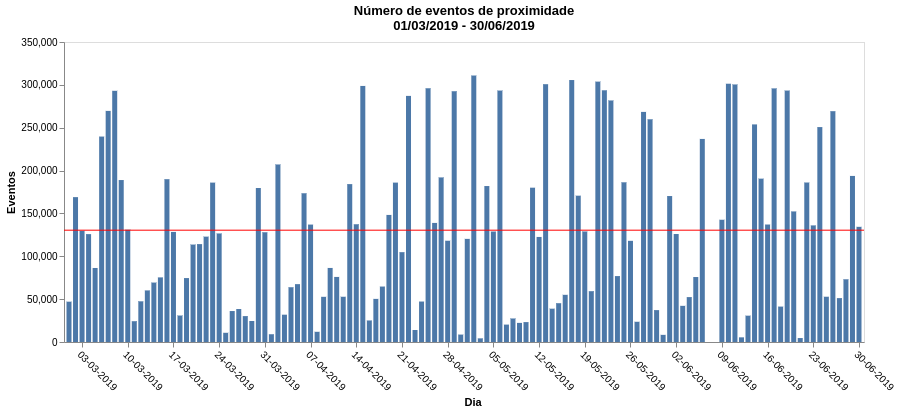
\includegraphics[width=.9\textwidth]{Capitulo4/img/eventos_proximidade.png}
\caption{Número de eventos de proximidade coletados no período de 01/03/2019 à 30/06/2019.}
\label{fig:eventos-de-proximidade}
\end{figure}


\ric{Figuras de centralidade parecem ser melhor apresentadas em mapas, onde se pode ver a localização dos pontos considerados.}

\begin{figure}
\centering
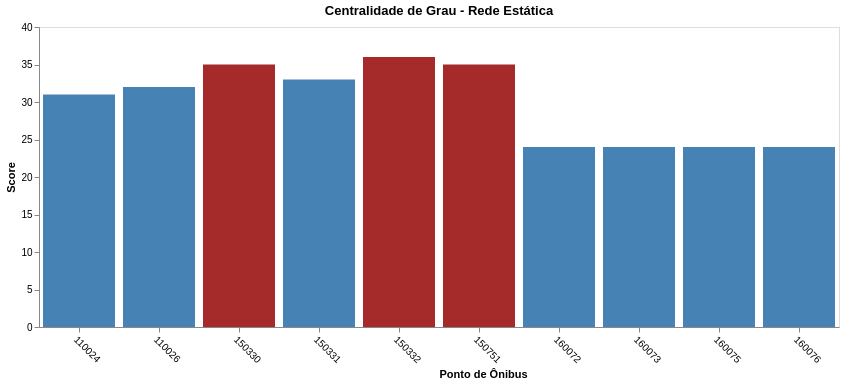
\includegraphics[width=.9\textwidth]{Capitulo4/img/centralidade-grau.png}
\caption{Centralidade de grau da rede estática.}
\label{fig:eventos-de-proximidade}
\end{figure}

\begin{figure}
\centering
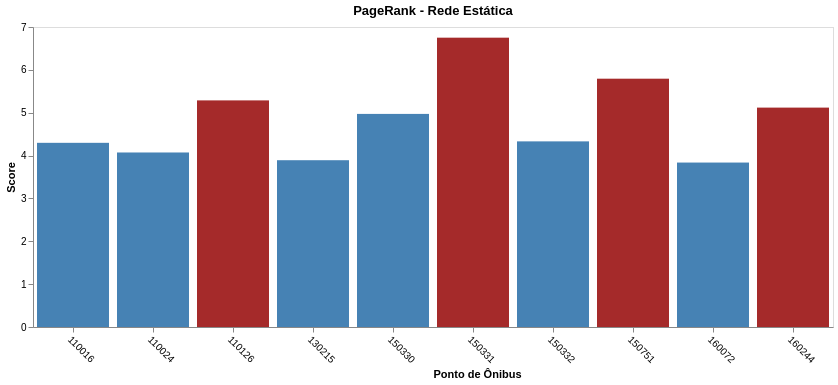
\includegraphics[width=.9\textwidth]{Capitulo4/img/pagerank.png}
\caption{PageRank da rede estática.}
\label{fig:eventos-de-proximidade}
\end{figure}


\begin{figure}
\centering
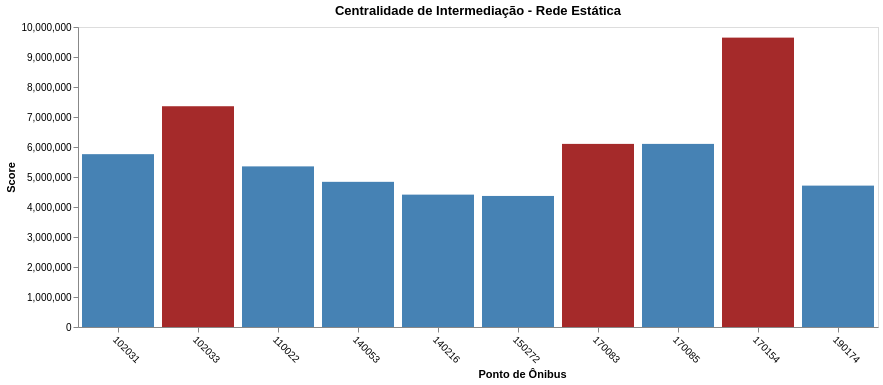
\includegraphics[width=.9\textwidth]{Capitulo4/img/centralidade-intermediacao.png}
\caption{Centralidade de Intermediação.}
\label{fig:eventos-de-proximidade}
\end{figure}



% Integração Temporal
% Os passageiros do transporte coletivo de Curitiba têm diferentes tipos de integração temporal para trocar de linha de ônibus ou de estação-tubo sem precisar pagar nova tarifa. Em 2017 foram mais de 600 mil usos nas integrações temporais das linhas urbanas da capital. Se contar o acesso às Ruas da Cidadania, esse atendimento sobe para quase um milhão.

% A proposta das integrações temporais no transporte é oferecer uma alternativa aos passageiros que ainda não têm acesso à integração no sistema. No transporte da capital, uma pessoa embarca num ponto e percorre todos os 21 terminais e as mais de 300 estações-tubo pagando apenas uma tarifa. Isso ocorre em 92\% da rede de transporte da cidade. A integração temporal busca complementar gradativamente essa rede.

% O único critério para usar a integração temporal é ter o cartão-transporte da URBS, que permite também o acesso às Ruas da Cidadania, onde o passageiro economiza uma tarifa no retorno ao ônibus. Veja quais são os tipos de integrações possíveis:

% Para o usuário ter direito à integração temporal, o mesmo deve utilizar o cartão-transporte da URBS em um dos validadores do Sistema de Transporte Coletivo de Curitiba (Ônibus, Terminal, Estação-Tubo), realizando assim um debito de passagem do seu Cartão Transporte e conforme as regras abaixo.

% OBS.: apenas os cartões-transporte nas modalidades Usuário e Estudante realizam integração temporal. Com o cartão-transporte Avulso não há a possibilidade de uso do benefício da integração temporal.


 
 
%\ric{Cada resultado precisa ser explicado.}

% A Figura~\ref{fig:centralidade-grau-estatica} mostra a centralidade de grau considerando apenas os pontos de ônibus (rede estática, ou seja, sem movimentação de ônibus). Os pontos 150331, 110026 e 150332 são os pontos de maior centralidade de grau, ou seja, conectam um número maior de pontos de ônibus devido a um maior número de linhas que passam por estes pontos. Em Curitiba, enquanto que o segundo ponto localiza-se na região central da cidade, os dois outros pontos (150331 e 150332) localizam-se na região sul da cidade. Em todos os casos, são pontos para onde convergem várias linhas de ônibus antes de chegarem a terminais importantes da cidade (terminal Pinheirinho ao sul, nos caso dos pontos 150331 e 150332, e praça Rui Barbosa no centro, no caso do ponto 110026). 
%Cabe ressaltar que a rede complexa construída considera pontos distintos, mesmo em terminais de ônibus, seguindo representação da URBS.

%{\bf Resultado 1:} Grau dos nós (\emph{Bus Stop}) para a rede estática (sem \emph{Stops}) na forma de histograma para os 10 nós de maior grau;

% \begin{figure}
% \centering
% \includegraphics[width=.9\textwidth]{fig/fig5.png}
% \caption{Centralidade de grau para pontos de ônibus (dez maiores) sem movimentação de ônibus (rede estática).}
% \label{fig:centralidade-grau-estatica}
% \end{figure}

% A Figura~\ref{fig:centralidade-grau-dinamica} mostra a centralidade de grau considerando as paradas de ônibus nos pontos de ônibus ao longo do dia (rede dinâmica, ou seja, com movimentação de ônibus). São mostrados os resultados para os três pontos de maior centralidade de grau da rede estática (150331, 110026 e 150332). Nota-se uma maior concentração no período da manhã e meio do dia, com diminuição gradual até o final da noite. Ao mesmo tempo, o ponto 150331 atende um elevado número de ônibus no período da manhã e no final da tarde. Essa última característica ocorre em Curitiba por conta do encerramento de atividades em empresas (trabalhadores retornando a suas casas) e estudantes de ensino noturno se deslocando para instituições de ensino.

%{\bf Resultado 2:} Evolução ao longo do dia do grau dos top 3 nós (\emph{Bus Stop}) anteriores;


% \begin{figure}
% \centering
% \includegraphics[width=.9\textwidth]{fig/fig7.png}
% \caption{Centralidade de grau para pontos de ônibus (três maiores) com movimentação de ônibus ao longo do dia (rede dinâmica)}
% \label{fig:centralidade-grau-dinamica}
% \end{figure}


% A Figura~\ref{fig:pagerank} mostra o \emph{page rank} considerando apenas a rede estática (pontos de ônibus). Os pontos 150331, 110026 e 110016 são os pontos de maior \emph{page rank}. Estes pontos se localizam, respectivamente, na região sul da cidade (na saída do terminal Pinheirinho), na região que conecta o centro a região nordeste da cidade (na direção de terminais Cabral, Boa Vista e Santa Cândida), nas proximidades do centro da cidade. Todos esses pontos conectam várias linhas que se afastam (pontos 150331 e 110126) ou se aproximam (ponto 11016) de regiões de grande concentração de pontos finais de linhas de ônibus. Ou seja, a importância destes pontos se deve a ligações com outros pontos importantes (pontos ou terminais com grande concentração de linhas).

%Lembrando que esta métrica indica relevância de pontos em relação aos demais pontos que se conectam a eles: são pontos importantes porque outros pontos significativos estão conectados, por linhas de ônibus, a eles.}

%{\bf Resultado 3:} \emph{PageRank} dos nós (\emph{Bus Stop}) para a rede estática (sem \emph{Stops}) na forma de histograma para os 10 nós de maior \emph{rank};

% \begin{figure}
% \centering
% \includegraphics[width=.9\textwidth]{fig/fig8.png}
% \caption{\emph{Page rank} para pontos de ônibus (dez maiores) sem movimentação de ônibus (rede estática).}
% \label{fig:pagerank}
% \end{figure}

%%%% Comentado por falta de espaço

% A Tabela~\ref{tab:n_linhas} mostra a comparação entre os três vértices de maior centralidade de grau (150332, 150331 e 110026) e os três vértices de maior \emph{page rank} (150331,150751,160244). \mar{Assim que os valores de grau forem recolocados, cabe um comentário sobre relação grau x page rank.}

% \begin{table}[h]
%     \caption{Comparação entre centralidade de grau  e \emph{page rank.}}
%     \label{tab:n_linhas}
%     \centering
%     \begin{tabular}{cccc} 
%         \hline
%         Ponto & Centralidade de grau & \emph{Page rank} \\
%         \hline
%         150332 & 63  & 4.15 \\
%         110026 & 64  &  3.75 \\
%         150751 & 63  & {\bf 5.53 } \\
%         150331 & 65  & {\bf 6.58} \\
%         160244 & 40  & {\bf4.82} \\
%         150330 &  32 &  4.75 \\
%         \hline 
        
%     \end{tabular}
% \end{table}

% \begin{table}[h]
%     \caption{Comparação entre Centralidade de grau  e \emph{page rank.}}
%     \label{tab:n_linhas}
%     \centering
%     \begin{tabular}{ccccc} 
%         \hline
%         Ponto & No. linhas & Centralidade de Grau & \emph{Page Rank} \\
%         \hline
%         110026 & 27  & 23 &  3.91 \\
%         150332 & 24  & 32 & 2.21 \\
%         150331 & 24  & 27 & {\bf 6.01} \\
%         110126 & 18  & 21 &  {\bf 5.50} \\
%         110016 & 16  & 11 & {\bf 4.57}\\
        
%         \hline  
%     \end{tabular}
% \end{table}

% As medidas de comprimento das linhas da rede estática de transporte resultaram em 40~m, 38,14~km e 9,43~km para os comprimentos mínimo, máximo e médio (com desvio padrão de 6,5~km) das linhas de ônibus. Já as medidas baseadas em caminhos mínimos entre pontos da rede resultaram em um valor mínimo de 3,6~m, diâmetro da rede (caminho mínimo mais longo) de 55~km e um percurso médio de 14,04~km. Estes caminhos mínimos foram obtidos através dos atributos de distância (\texttt{DISTANCE}) das arestas \texttt{NEXT\_STOP}, gerando uma rede ponderada do sistema de transporte de Curitiba. Note que esse percurso médio pode ou não ser factível com troca de ônibus (baldeação), dependendo da origem e destino do passageiro.
%Tais métricas são úteis para comparação entre sistemas de transporte de diferentes cidades, e para planejamento do próprio sistema, seja na redução de distância ou no tempo de percurso dos passageiros.

%{\bf Resultado 5:} Tabela de medidas da rede estática: comprimento mínimo, máximo e médio das linhas (em km); média dos caminhos mínimos (de cada nó para todos os outros; diâmetro da rede (caminho mínimo mais longo);


% \begin{table}[h]
%     \caption{Comprimento das linhas de ônibus e diâmetro da rede estática (km).}
%     \label{tab:medidas}
%     \centering
%     \begin{tabular}{cccc} 
%         \hline
%       Mínimo &Máximo &Médio (desv. padrão) &Diâmetro\\
%         \hline
%         0,04 & 38,14  & 9,43 (6,5) & xxx \\
%         \hline  
%     \end{tabular}
% \end{table}

% A Figura~\ref{fig:betweeness} mostra a centralidade de intermediação considerando apenas a rede estática (pontos de ônibus). Os pontos 170154, 170085 e 170083 são os pontos de maior centralidade de intermediação. Estes pontos localizam-se na vizinhança do terminal Pinheirinho, localizado na parte sul de Curitiba, comportando-se como um \emph{hub} por onde passam percursos mais curtos entre pontos de ônibus da rede. Note também que esses percursos podem ou não ser factíveis com trocas de ônibus.
%Eles refletem indiretamente a movimentação de pessoas dessa região da cidade (basicamente bairros-dormitórios) para trabalharem ou estudarem nas demais partes da cidade, ou seja, a uma relação desses resultados com a evolução urbana da cidade.

%{\bf Resultado 6:} Centralidade de intermediação (\emph{betweenness}) - ver depois.

% \begin{figure}
% \centering
% \includegraphics[width=.9\textwidth]{fig/fig9.png}
% \caption{Centralidade de intermediação para pontos de ônibus (dez maiores) sem movimentação de ônibus (rede estática).}
% \label{fig:betweeness}
% \end{figure}


% \begin{table}[h]
%     \caption{PageRank 07:00 - 10:00 02/05/2019}
%     \centering
%     \begin{tabular}{llll} 
%         \hline
%         ID Ponto	 &No. linhas &No. paradas &PageRank  \\
%         \hline
%         150751 &24 &1440 &2.74556 \\
%         150331 &24 &1152 &3.43579 \\
%         110026 &26 &704  &2.68251 \\
%         110024 &26 &496  &2.89234 \\
%         150635 &14 &418  &2.67968 \\
%         160244 &17 &160  &2.88967 \\
%         190199 &7  &143  &2.69128 \\
%         150203 &5  &143  &2.63893 \\
%         120020 &8  &72   &2.76218 \\ 
%         190198 &6  &9	 &2.75211 \\
%         \hline 
%     \end{tabular}
%     \label{tab:res_pagerank_07_10}
% \end{table}



% \begin{table}[h]
%     \caption{PageRank 07:00 - 10:00 02/05/2019}
%     \centering
%     \begin{tabular}{ llllll } 
%         \hline
%         Nº doPonto	 & Nome do Ponto &	linhas & N° Veículos & Nº Paradas &	PageRank  \\
%         \hline
%         150751 & 	Av. Winston Churchill, 2677     &	24 & 21 & 1440 & 2.74556 \\
%         150331 &	 Av. Winston Churchill, 2472    &	24 & 19	& 1152 & 3.43579 \\
%         110026 &	 Rua Alferes Poli, 400          &	26 & 16	& 704  & 2.68251 \\
%         110024 &	 Rua Alferes Poli, 787          &	26 & 13	& 496  & 2.89234 \\
%         150635 &	 Av. Pres. Getulio Vargas, 2676 &	14 & 15	& 418  & 2.67968 \\
%         160244 &	 Rua Emanoel Voluz, 284         &	17 & 5	& 160  & 2.88967 \\
%         190199 &	 Marginal Rodovia BR- 277, 926  & 	7  & 6	& 143  & 2.69128 \\
%         150203 &	 Rua Alcino Guanabara, 1237     & 	5  & 7	& 143  & 2.63893 \\
%         120020 &	 Av. Anita Garibaldi, 3431      &	8  & 6	& 72   & 2.76218 \\ 
%         190198 &	 Marginal Rodovia BR- 277, 926  &	6  & 1	& 9	   & 2.75211 \\
%         \hline 
%     \end{tabular}
%     \label{tab:res_pagerank_07_10}
% \end{table}


% \begin{table}[h]
%     \caption{PageRank 12:00 - 14:00 02/05/2019}
%     \centering
%     \begin{tabular}{ llllll } 
%         \hline
%         Nº do Ponto	 & Nome do Ponto &	linhas & N° Veículos & Nº Paradas &	PageRank  \\
%         \hline
%         150751 & Av. Winston Churchill, 2677      &	24	& 21 & 1440 & 2.64988  \\
%         150331 & Av. Winston Churchill, 2472      &	24	& 19 & 1152	& 2.85910  \\
%         110026 & Rua Alferes Poli, 400	          & 26	& 16 & 704	& 2.47933  \\
%         110024 & Rua Alferes Poli, 787	          & 26	& 13 & 496	& 2.64934  \\
%         160244 & Rua Emanoel Voluz, 284 	      & 17	& 5	 & 160	& 2.79724  \\
%         180020 & Rua Rezala Simão, 997            &	 7	& 6	 & 143	& 2.95418  \\
%         190199 & Marginal Rodovia BR- 277, 926    &  7	& 6	 & 143	& 2.42175  \\
%         150203 & Rua Alcino Guanabara, 1237       &	 5	& 7	 & 143	& 2.38609  \\
%         150070 & Rua Maria Trevisan Tortato, 642  &  7	& 3	 & 52	& 3.02172  \\
%         180007 & R. Carlos Klemtz, 1000           &	 7	& 4	 & 52	& 2.72499 \\
%         \hline 
%     \end{tabular}
%     \label{tab:res_pagerank_12_14}
% \end{table}


% \begin{figure}
% \centering
% \includegraphics[width=.9\textwidth]{fig/fig2.png}
% \caption{Evolução horária do grau da rede do sistema de transporte no dia 02/05/2019}
% \label{fig:grau}
% \end{figure}


% \begin{figure}
% \centering
% \includegraphics[width=.9\textwidth]{fig/fig3.png}
% \caption{nº de veículos no dia 02/05/2019}
% \label{fig:veiculos}
% \end{figure}



\section{Integração temporal}

%%%%%% O que está abaixo não necessariamente permanecerá no texto - por enquanto é apenas uma referência para a seção

\ric{Resumo da metodologia}

\begin{enumerate}
    \item Para cada ponto de ônibus, obtém-se uma série temporal com o número de eventos (paradas de ônibus) em uma janela deslizante de 10 min, calculada minuto a minuto ao longo do período considerado (0 a 24 horas?);
    \item Identificam-se os 10 pontos (centroides) mais bem servidos em termos do número de eventos agregados para todos o período considerado;
    \item Para cada centroide, selecionam-se os pontos a uma distância de 600~m do centroide e gera-se uma matriz de correlação entre as séries temporais de cada ponto desta região;
    \item Identificam-se os pontos de maior correlação (com o centroide?);
    \item Estes pontos serão os candidatos para estabelecer integração temporal.
\end{enumerate}

\ric{Resultados a serem apresentados sobre o levantamento de regiões candidatas para integração temporal:}

\begin{itemize}
    \item Visualização das regiões estudadas (centroides) no mapa de Curitiba;
    \item Número de pontos e raio médio destas regiões, ou seja, os pontos selecionados estão em um raio muito menor do que 600~m?
    \item Quantas linhas de ônibus servem cada região? Elas se conectam em algum outro ponto da rede, ou seja, existe um terminal ou estação tubo onde a transferência possa ser realizada ser pagamento de nova tarifa?
    \item Dar especial atenção aos centroides que "integram" várias linhas (Alferes Poli?; Centro Cívico?); estes centroides, além de possuírem serviços "sincronizados" (precisa definir o que seria isso), permitem criar novas rotas;
\end{itemize}

\ric{Resultados a serem apresentados sobre o impacto na rede da implementação da integração temporal para as regiões selecionadas:}

\begin{itemize}
    \item Tem impacto na métrica de redes complexas (centralidade de proximidade ou intermediação, diâmetro)?
\end{itemize}